In order to evaluate the approach proposed in this paper, we have collected
a dataset with a car in an urban setting. Our car is equipped with a Sony
XCD-SX910 camera recording $1280$x$960$ images at $3.75$ frames per second and
an XSens MTi IMU running at $100$ Hz with $x$ pointing forward, $y$ to the
right, and $z$ upward. The sequence contains $8218$ images and lasts around $40$
minutes. We have encountered different scenes comprising of traffic lights,
crosswalks, or changes of speed limit. We have driven in a loop so as to come
several times in the same situation and thus have an estimation of the quality
of our solution.

\subsection{Simulation}
Since it is easier to have a ground truth on simulated data and hence validate
our approach, we first display an experiment of the whole algorithm on synthetic
data. For visualization purposes, we have simulated IMU data with an univariate
normal distribution and have introduced change-points every $50$ data points. We
have randomly generated 3 different $\boldsymbol{\alpha}_i$ with $K=256$ coding
for the traffic situations. Although the algorithm starts with no prior
knowledge, we could also start with previously learned models $M_i$ and $A_i$.

Fig.~\ref{fig:simulation} depicts the output of the simulation and demonstrates
the pertinence of our method. We display the MAP solution for \eqref{eqn:action}
on the bottom plot and thus the prediction reflects the Gaussian with the
maximum number of data points. At time step $100$, a new Gaussian with mean
$10$ is created for label $2$. It becomes the MAP only at time step $300$ after
accumulating enough evidence. Even though the label numbers $l_t$ differ from
the ground truth, they are actually correctly estimated since the induced
partition is equivalent.

\begin{figure}[t]
\centering
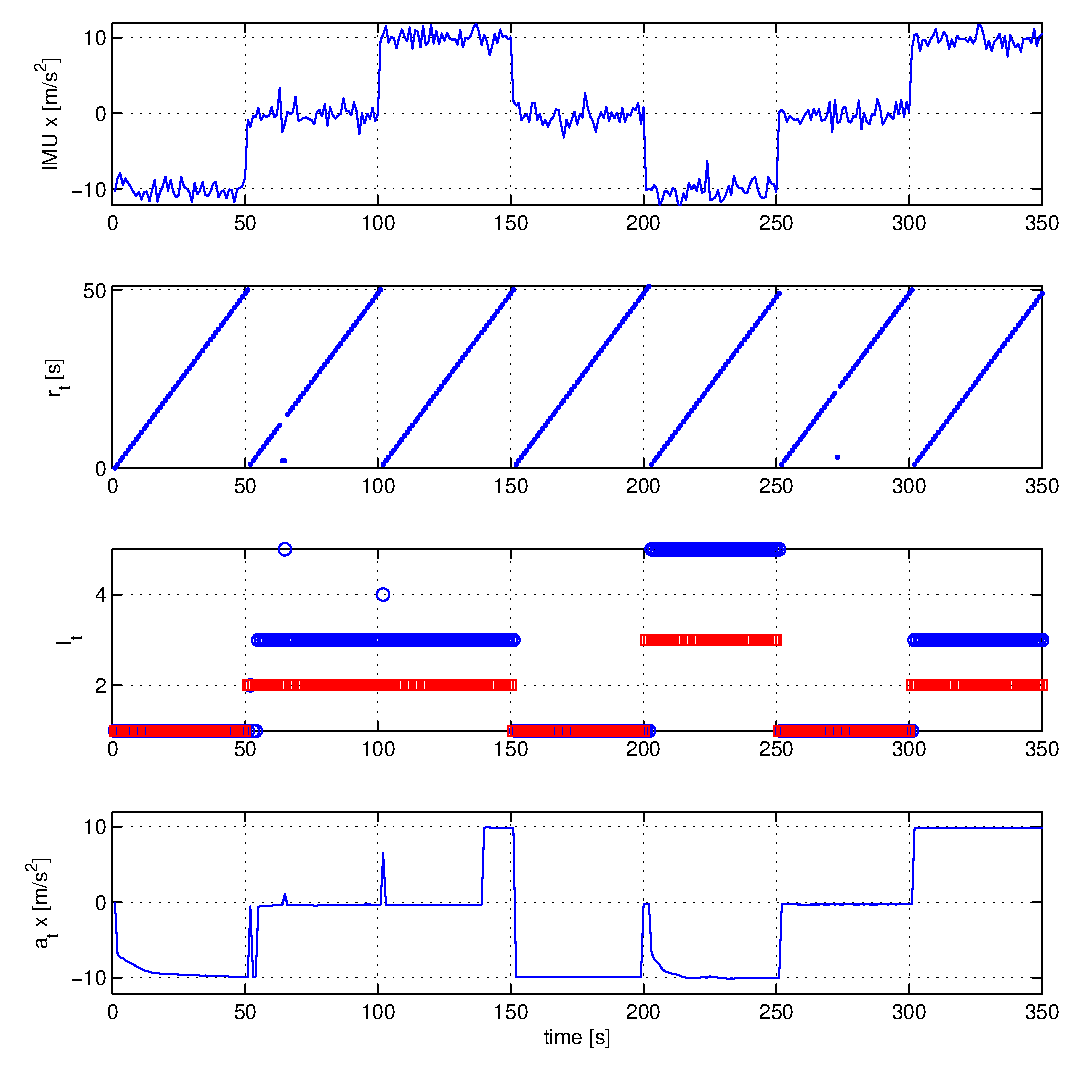
\includegraphics[width=0.8\columnwidth]{fig/simResult.eps}
\caption{Simulation results of the algorithm. From top to bottom, the
  plots display the simulated IMU data $\mathbf{z}_t$, the inferred
  segment lengths $r_t$, the inferred labels $l_t$ (blue circle) with
  ground truth (red square), and the MAP estimate for the action
  $\mathbf{a}_t$.\vspace{-5mm}}
\label{fig:simulation}
\end{figure}

\subsection{Motion Segmentation}
We have estimated the quality of our motion segmentation algorithm
from Section~\ref{sec:motion} on real-world data and performed inference on the
final posterior distribution \eqref{eqn:joint} to get the optimal
sequence of segment lengths which represents our motion segments. We set the
hazard rate to $\lambda=1/10$, the number of particles to $P=100$, and the prior
hyperparameters of the normal-Wishart to $\kappa_0=1,
\boldsymbol{\rho}_0=\mathbf{0},\nu_0=3,\boldsymbol{\Lambda}_0=\mathbf{I}$. We
only considered IMU data at $10$ Hz.

Fig.~\ref{fig:motion_segments} shows the extracted motion segments along with
the corresponding IMU data. Our algorithm identified $165$ segments which are
validated by visual inspection of the IMU data. Furthermore, the segmentation
has been compared to a manual annotation of our image sequence and exhibited an
accuracy of approximatively $92\%$. For the labeling of the change-points, we
have watched the video and noted down where we would expect a change of driving
behavior. The parameter $\lambda$ controls the false positives/negatives rates.

\begin{figure}[t]
\centering
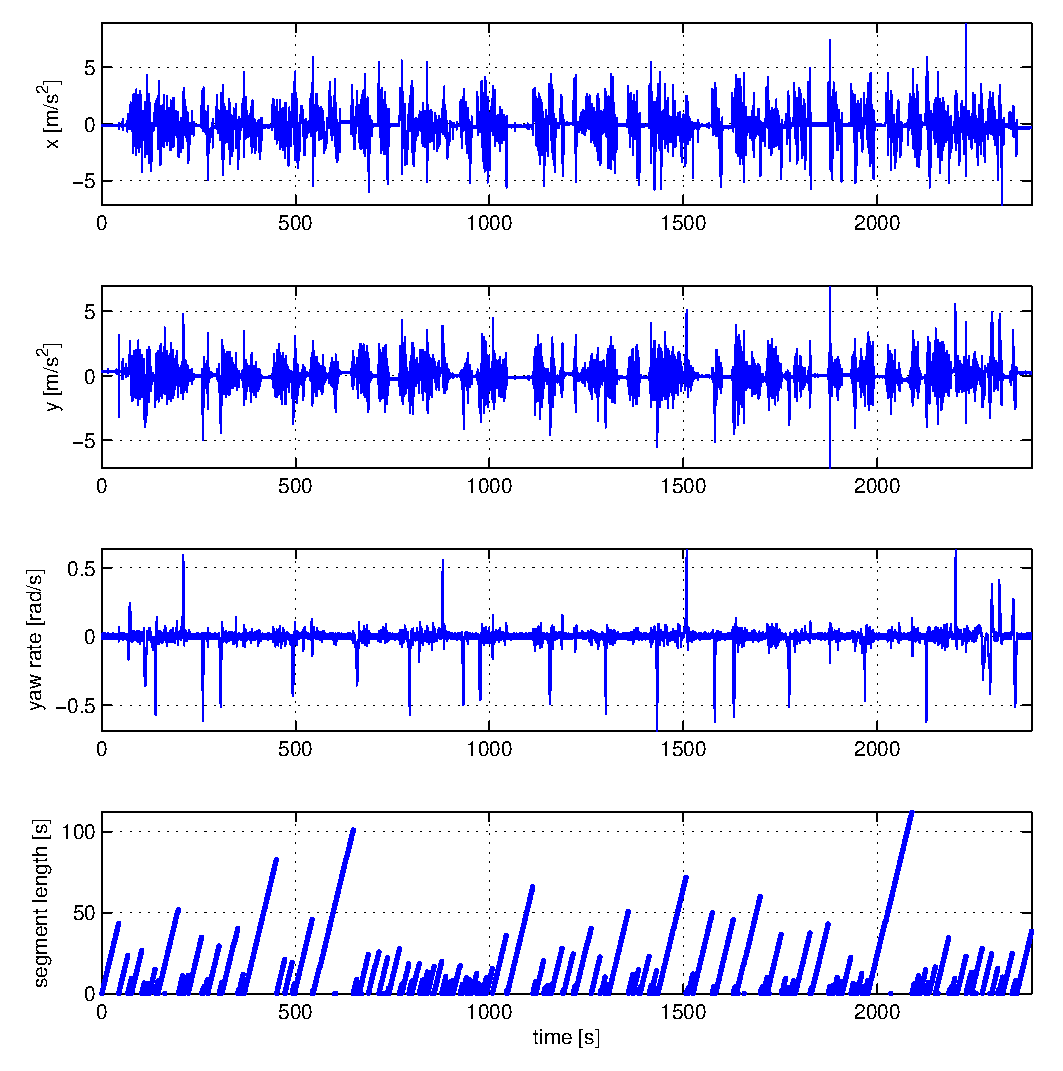
\includegraphics[width=0.770576\columnwidth]{fig/cpResult.eps}
\caption{Optimal motion segmentation from IMU data. The three top plots are the
IMU raw values over time. The bottom plot depicts the motion segments
discovered by our algorithm.\vspace{-5mm}}
\label{fig:motion_segments}
\end{figure}

\subsection{Traffic Situation Labeling and Recognition}
We have evaluated the technique presented in Section~\ref{sec:labeling} and
performed inference on \eqref{eqn:labeling} to obtain the most likely label for
a scene. In a first phase, we have collected a subset of images from traffic
lights, yield signs, and pedestrian crossings. Models $M_i$ were learned on
these images using \eqref{eqn:alpha_update} and frozen during the evaluation. In
a second phase, we have started the algorithm with no prior models. The
dictionary was created from a set of $N=400$ randomly picked images and the SIFT
features quantized into $K=256$ visual words. The prior hyperparameters of the
Dirichlet distribution were set to $\boldsymbol{\alpha}_0=\mathbf{1}$.

In the supervised case, we have manually annotated the image sequence and
compared the resulting labeling to the ground truth. We obtained an
accuracy of $93\%$ for traffic light scenes, $99\%$ for yield scenes, and
$91\%$ for pedestrian crossings scenes. We except these results to drop slightly
in a previously unseen environment. In the unsupervised case, $\xi$ acts as a
concentration parameter, i.e., it controls the tendency to create new classes.
The final labeling is challenging to evaluate. Two traffic lights
scenes might for instance get different labels without interfering into the
final action prediction. With $\xi=200$, our algorithm discovered $15$ different
traffic situations and was able to re-associate correctly to the same labels in
the different runs of our driving loop.

\subsection{Action Prediction}
The strategy presented in Section~\ref{sec:action} is relatively straightforward
to evaluate, since predictions can be compared to incoming IMU data. We set the
threshold for creating a new Gaussian to $\epsilon=5$ and inferred on
\eqref{eqn:action}. Our algorithm performed accurately in predicting the driving
actions.
